%===================================== CHAP 7 =================================

\chapter{Project Life Cycle}
This chapter includes the life cycle of the project, describing each phase of the process.

\section{Planning}
The group initiated the project with a planning and research phase, lasting from January the 11th to February the 3rd. 

The importance of the planning phase was emphasized by the group to avoid being forced to start over because the project was insufficient according to what the customer wanted.

The planning phase was initiated by thoroughly choosing the right project, focusing on the strengths and weaknesses within the group. To ensure that every member had the same ambitions and a common understating of what the group expected of each other, a group contract was also formulated. This contract has been important for the group dynamic, see Appendix \ref{group_contract}. The risk analysis was also developed during the planning phase, as issues might arise unexpectedly and need to be managed in a proper fashion. The risk analysis was used to prevent and mitigate issues that happened.  

As the project was assigned, the group prioritized to establish contact with the customer to get a more precise idea of what was to be developed. A contract between the team and the customer was also formulated, ensuring both parties had the same expectations for the project and each other during the development process, see Appendix \ref{customer_contract}.

As the group achieved a greater idea of what the project implied, a set of roles were created. These were delegated to the group members depending on prior experience and wishes.

Detailed information about each sprint can be found in Appendix \ref{Sprints}.


\section{Sprint 0}
\label{sprint0}
The sprint goal for sprint 0 was "Planning, set up product backlog and create a first draft of the design". Sprint 0 did not consist of any user stories. The sprint main focus was to make sure the development of the product could start in sprint 1. 

This included:
\begin{itemize}[noitemsep]
    \item Set up workspace
    \item Create index template in Django
    \item Create product backlog with customer
    \item Define MVP (see section \ref{MVP})
    \item Create a first design draft of the application
    \item Planning
\end{itemize}


\section{Sprint 1}
\label{sprint1}
The sprint goal for sprint 1 was to "Deliver first interactive prototype to customer". To achieve this goal, the group created milestones during the sprint planning, defining what should be finalized during the iteration. 

The milestones were as as follows:
\begin{itemize}[noitemsep]
  \item Create a mock up database.
  \item Create a flow diagram.
  \item Create issues on GitHub.
  \item Make log in, with different GUI for each role (child, parent, activity      provider, maintainer and anonymous).
  \item Log in with Facebook.
  \item Anonymous user should maybe not be able to see who is going to a activity anonymous should not be able to sign up for activity, before the user has logged in.
  \item Site map
  \item Create skeleton for all pages in site map
  \item Update wiki (to have the flow diagram, site map and user manual)
\end{itemize}
 
Two problems were encountered during this sprint. Firstly, one group member asked for five days off to travel, this is discussed in Appendix \ref{Sprints-sprint1}. The second problem encountered was a misunderstanding between the group and the customer, specifically the definition of proof of concept. The group thought that the web portal should include all functionalities, as a system ready for production. The customer, on the other hand, wanted the design of the concept fully completed but not necessarily a fully functional web portal. The group resolved this with a new meeting with customer and a technical manager at SINTEF Digital, and discussed the groups possibilities. At the end of the meeting the customer and the group agreed on using a web-server, see Appendix \ref{webhotel_vs_webserver}.


\section{Sprint 2} 
\label{sprint2}
The goal for sprint 2 was to implement functionality on the activities page; allowing the user to create and retrieve events, as well as filter these. 

The milestones in sprint 2 were as follows:
\begin{itemize}[noitemsep]
  \item Log in.
  \item Fill database.
  \item Create events.
  \item Retrieve events.
  \item Filter events.
  \item Sign up for event.
\end{itemize}

The group experienced a couple of problems during this sprint. First of all, the group came across problems trying to implement asynchronicity when filtering activities. Initially the group had chosen to use Flux, to manage the data flow in the application \cite{flux}. Midway in the sprint the group decided to use Redux. Due to these issues the milestone, filter events, had to be relocated to sprint 3. The customer also requested a first version of the web portal, therefore the group had to allocate resources to complete this. See detailed information about the sprint in Appendix \ref{Sprints-sprint2}.


\section{Sprint 3}
\label{sprint3}
The main goal for this sprint was to implement user interaction with the events on the web portal. Two milestones from the previous sprint, containing several issues, were included to this sprint. There was a focus on making the web portal easy to install. 

The milestones were as as follows: 
\begin{itemize}[noitemsep]
    \item Filter events (from sprint 2)
    \item Sign up for event (from sprint 2)
    \item Acceptance Tests
    \item Write User Test
    \item My Page
    \item Create an installation for customer
    \item Create an installation guide
    \item Display active users in navigation bar
    \item Workshop
\end{itemize}

The group was very effective this sprint and a lot of work were completed (see figure \ref{Activity_Plan}, \ref{Burndown_Sprint3} and \ref{Hours_Diagram_Sprint3}). No major problems were encountered and the minor problems were quickly resolved by asking the other team members for help. The group finalized the remaining issues from the previous sprint. 

In this sprint, plans were made to conduct usability and acceptance testing of the web portal. Because of overlapping schedules with the group, the customer and the test subjects, the workshops had to be postponed to the next sprints.

\begin{figure}[ht]
\centering
    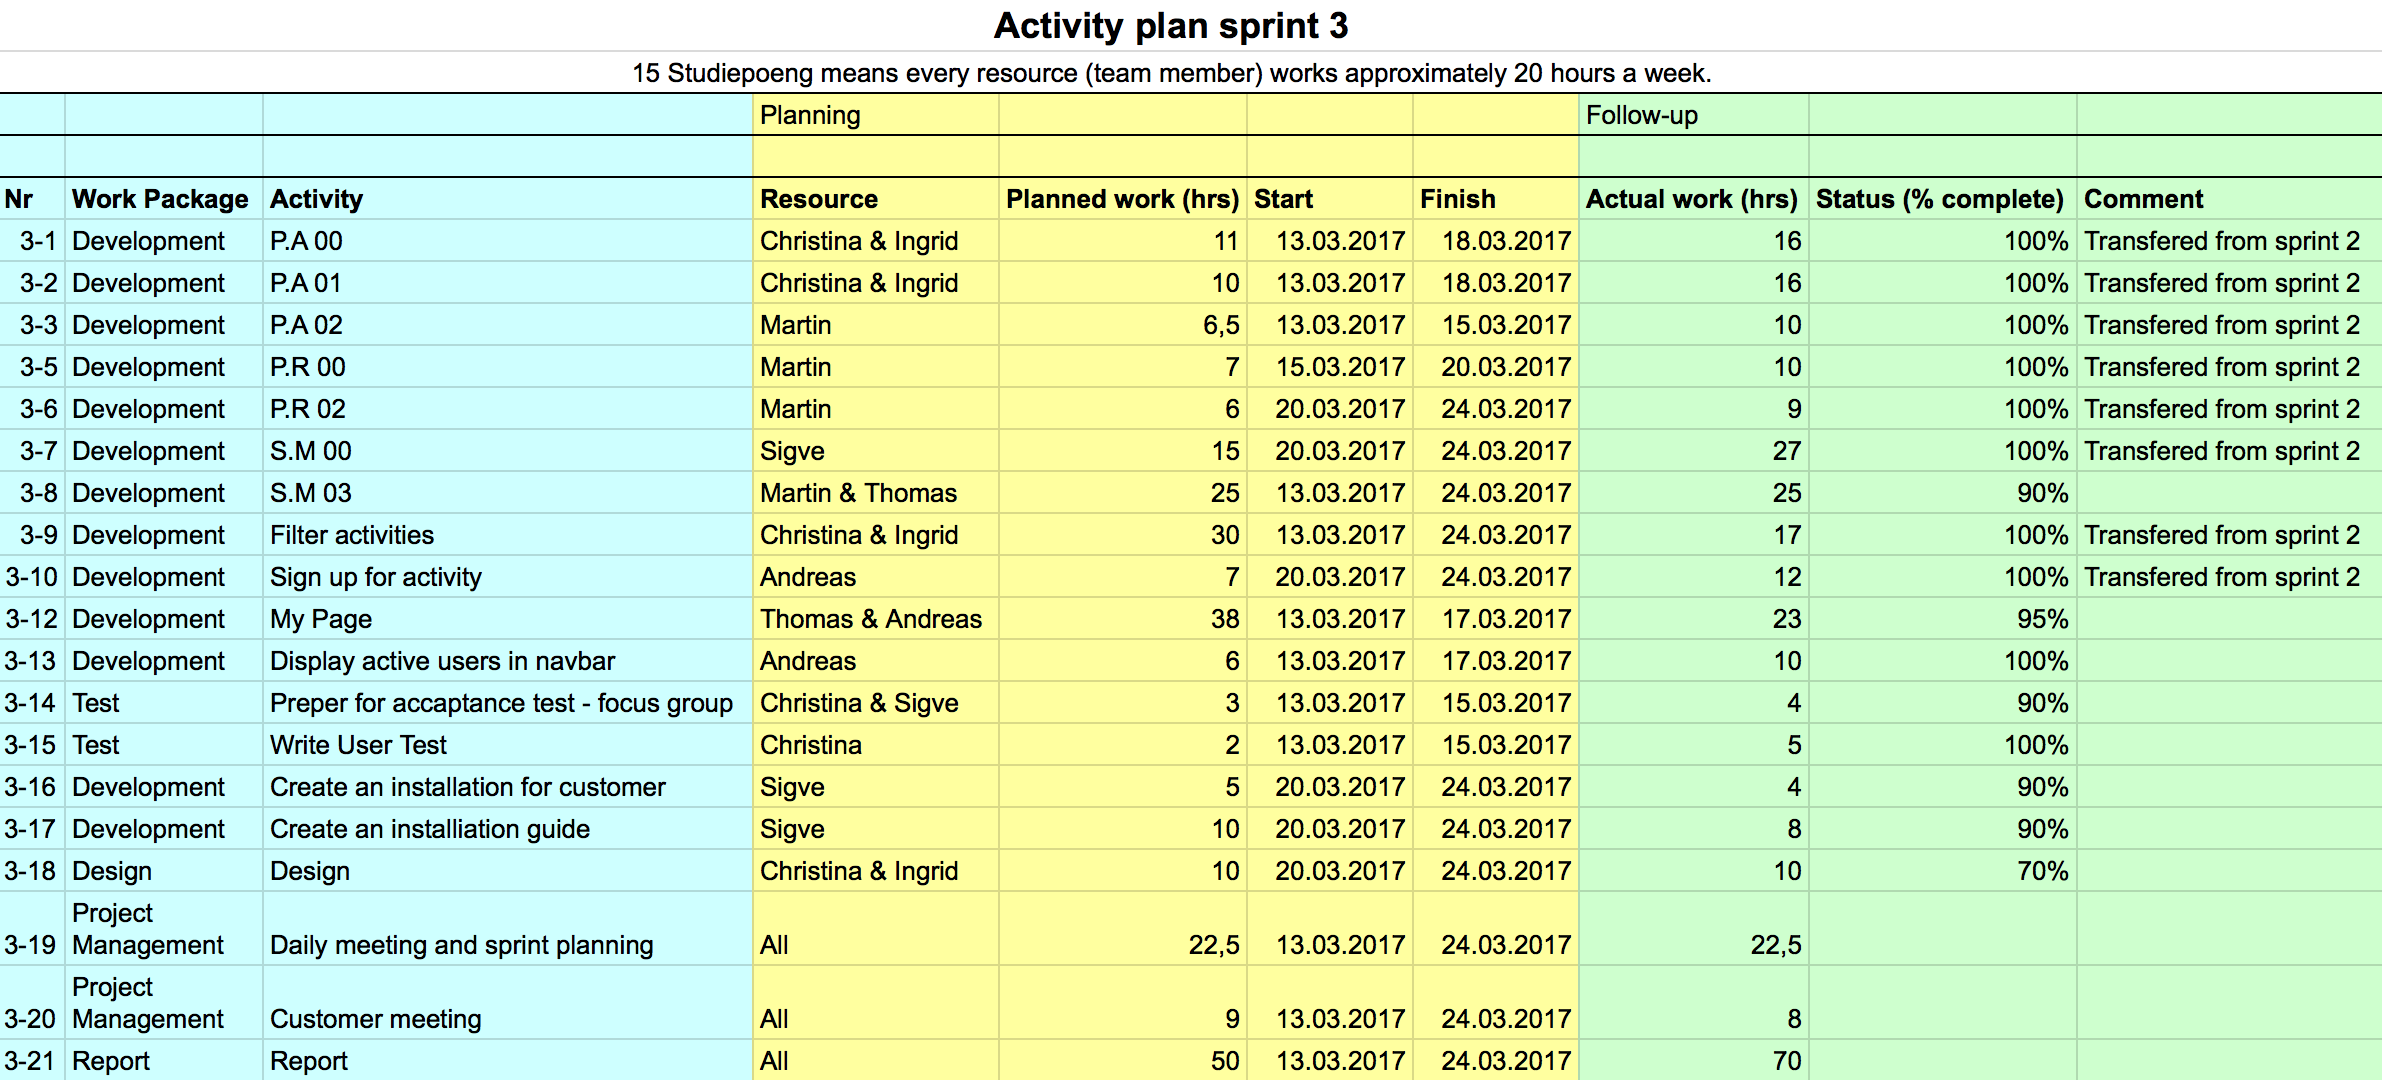
\includegraphics[angle=90,height=150mm,width=\textwidth]{fig/activity_plan_3}
\caption{Sprint 3 - Activity}
\label{Activity_Plan}
\end{figure}

\begin{figure}[ht]
\centering
    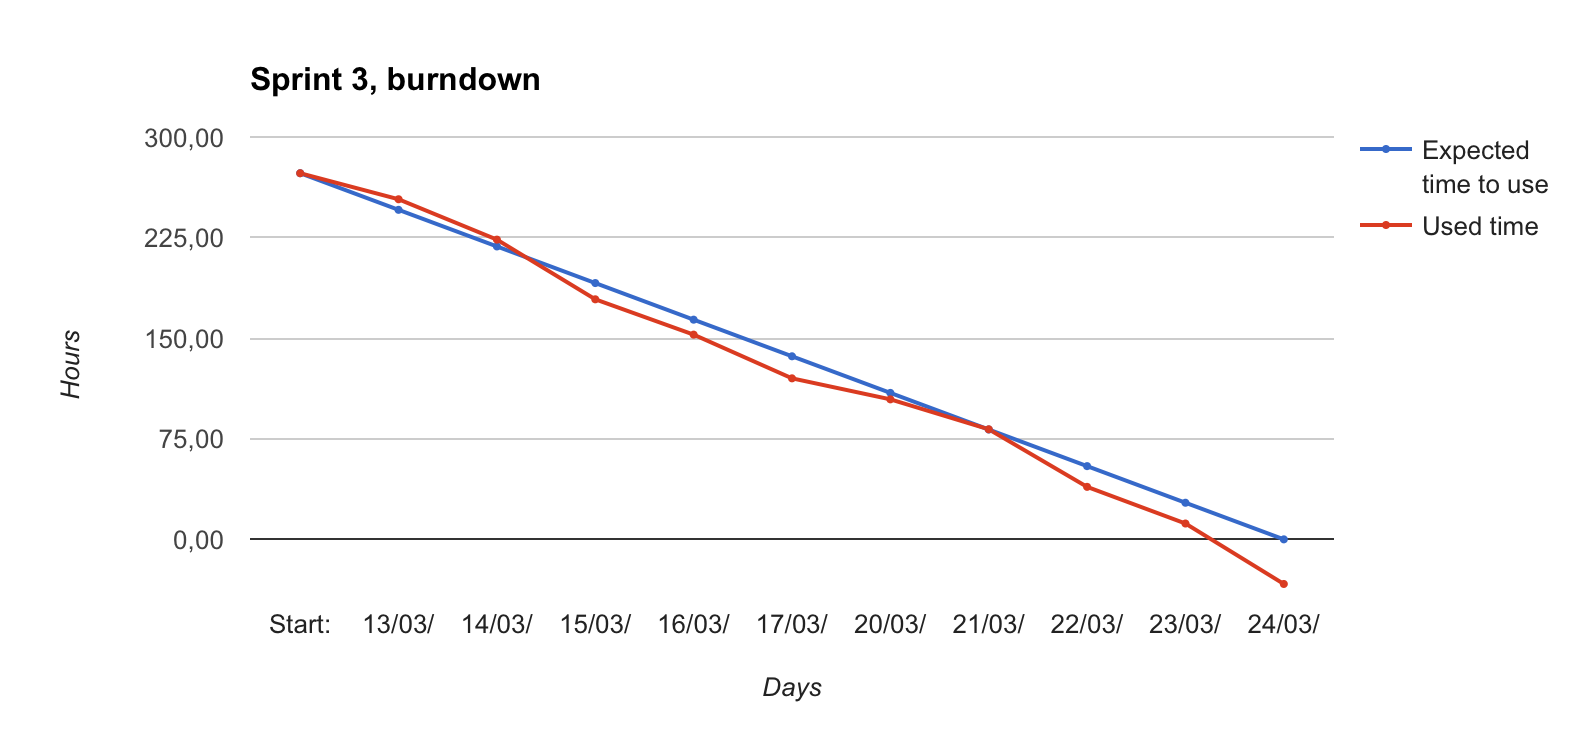
\includegraphics[width=0.8\textwidth]{fig/sprint3}
\caption{Sprint 3 - Burndown}
\label{Burndown_Sprint3}
\end{figure}

\begin{figure}[ht]
\centering
    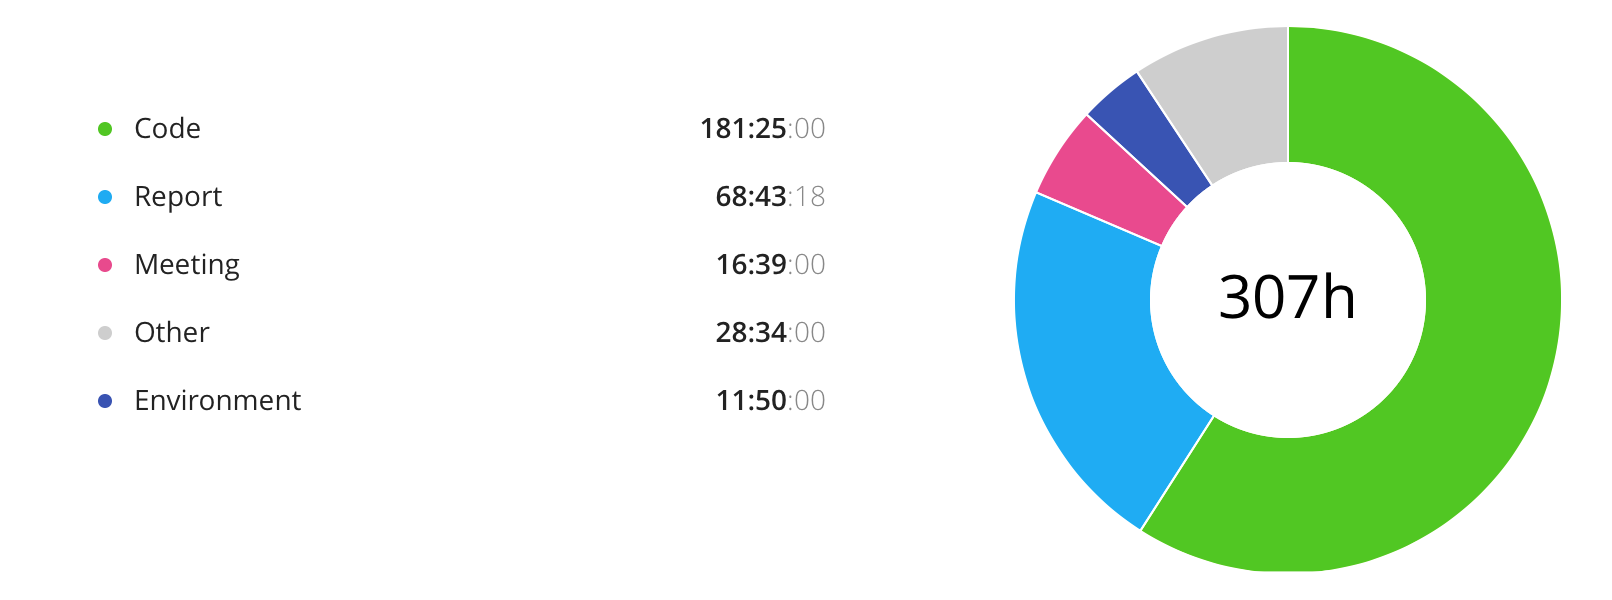
\includegraphics[width=0.8\textwidth]{fig/sprint3-diagram}
\caption{Sprint 3 - Distributed Time}
\label{Hours_Diagram_Sprint3}
\end{figure}

\section{Sprint 4}
\label{sprint4}
The main goal for this sprint was to implement and finalize the last product features. Making it possible for a user to represent and see information about providers, and test the web portal with focus groups.  

The milestones were as as follows: 
\begin{itemize}[noitemsep]
    \item Acceptance Test/focus-group test
    \item Facebook sign in
    \item Adaptions from DB
    \item Filter Activities
    \item User represent provider 
    \item Provider Page
    \item My Page, 
    \item Installation guide, 
\end{itemize}

During the sprint planning, the group went through the product backlog once more and prioritized and re-estimated the workload. The group had previously decided that sprint four was the last sprint where the group could implement new features (see section \ref{s:sprints}). The group conducted a focus-group test with providers and possible system maintainers. More information about sprint 4 and figures can be found in Appendix \ref{Sprints-sprint4}.


\section{Sprint 5}
\label{sprint5}
This sprint was used to finalize the product and make it ready to deliver to the customer. It was therefore decided not to implement any new features, but to focus on the existing product and fix current features. 

The focus group with the families were conducted during this sprint. After the focus group, the group and customer met to discuss the feedback. The feedback opened for many new ideas and constructive thoughts about design and features (see section \ref{proposal_for_future_features}). More information about sprint 5 and figures can be found in Appendix \ref{Sprints-sprint5}.


\section{Sprint 6}
\label{sprint6}

In sprint 6 the group finalized the report and prepared for demonstration of the product. The preparations included creation of both a poster and a movie, that presented the product. The movie can be found at \url{https://www.youtube.com/watch?v=Wak_BpixYbY}. Figures and poster can be found in Appendix \ref{Sprints-sprint6}

\cleardoublepage